\section{Intel Quantum Simulator on Kay}
\label{sec:intel_quantum_simulator_on_kay}

%---------------------------------------------------------------------------------
\subsection{Installation Setup}
\label{sec:installation_setup}
The Irish national supercomputer (Kay) was installed in August 2018, is operated by ICHEC and is comprised of
\begin{itemize}
    \item a 336 node cluster.
    \item 13,440 CPU cores, 63 TB distributed memory.
    \item Dual-socket 20-core Intel Xeon Gold (Skylake) 6148 at 2.4 GHz with 192 GB memory.
    \item 400 GB local SSD scratch.
    \item 100 GB Intel OmniPath network.
    \item Additional partitions
    \begin{itemize}
        \item Intel Xeon Phi (Knights Landing architecture).
        \item High-memory 1.5 TB RAM with 1TB local SSD scratch.
        \item Dual NVIDIA Tesla V100.
    \end{itemize}
\end{itemize}

The \textit{master} branch of the Intel Quantum Simulator from the \href{https://github.com/intel/Intel-QS/tree/master}{intel/Intel-QS} GitHub repository was installed on Kay in the path \texttt{/ichec/work/ichec001/}. The simulator was built with Intel Parallel Studio XE 2018 update 4 and vectorisation was enabled using AVX512 instead of the default SSE2.

%---------------------------------------------------------------------------------
\subsection{Performance and Scaling}
\label{sec:performance_and_scaling}
Testing was conducted using the \textit{tests/qft\_test.cpp} application supplied with the simulator which conducted a quantum Fourier transform using a specified number of qubits. Experiments were conducted for this application to demonstrate its weak and strong scaling performance. Due to the large memory footprint of the number of states, which doubles as the number of qubits increases by one, and the overhead of the corresponding access of that memory, the application was expected to be memory bound, and thus have relatively good weak scaling performance. As the number of quantum gate operations is increased in a quantum circuit the number of classical gates required to conduct the simulation can increase very quickly since these quantum gates are applied to an increasing number of qubits. Therefore, as the number of qubits are increased, the number of classical operations would increase significantly. Thus applications on the Intel Quantum Simulator are also subject to being compute bound.

Table \ref{tab:scaling_experiment_config} details the configuration of each experiment for both strong and weak scaling using double and also single precision numbers to represent the states. Figure~\ref{fig:strong_scaling} illustrates the results of the strong scaling performance and Figure~\ref{fig:weak_scaling} that of the weak scaling experiments.
Both Figure~\ref{fig:strong_scaling} and Figure~\ref{fig:weak_scaling} appear to scale approximately in a linear fashion. This implies that the application scaled relatively well for both weak and strong scaling. However, it would be desirable to conduct more experiments for larger problem sizes to further observe the scalability of the application. This was not possible due to the previously mentioned limit of the MPI message size.
% It must also be noted that the double precision performance for weak scaling was notably worse than that of single precision. However, it appears to perform worse by approximately the addition of a constant, which does not prove to be a significant issue.

\begin{table}[H]
\centering
    \begin{tabular}{|c|c|c||c|c||c|c|}
        \hline
        \multicolumn{3}{|c||}{Scaling} & \multicolumn{2}{|c||}{Strong} & \multicolumn{2}{|c|}{Weak}\\
        \hline
        Nodes           &  p    & NumProcs   & Local States  & Qubits      & Local States & Qubits \\
                   &     &  $2^p$  &  $ 2^{n-p}$  &   $n$      & $ 2^{n-p} = 2^{27}$ &  $n$\\
    
        \hline
        1               &   1   & 2                     & $2^{28-1}$                        & 28         &$2^{28-1}$&  28\\
        2               &   2   & 4                     & $2^{28-2}$                         & 28        &$2^{29-2}$&  29 \\
        4               &   3   & 8                     & $2^{28-3}$                         & 28        &$2^{30-3}$&  30 \\
        8               &   4   & 16                    & $2^{28-4}$                         & 28        &$2^{31-4}$&  31 \\
        16              &   5   & 32                    & $2^{28-5}$                         & 28        &$2^{32-5}$&  32 \\
        32              &   6   & 64                    & $2^{28-6}$                         & 28        &$2^{33-6}$&  33 \\
        64              &   7   & 128                   & $2^{28-7}$                        & 28         & $2^{34-7}$& 34 \\
     \hline
    \end{tabular}
    \caption{Details of number of total qubits, and local number of states per process for the corresponding experiment for both strong and weak scaling. }
    \label{tab:scaling_experiment_config}
\end{table}

\begin{figure}[H]
	\centering
	\begin{minipage}{.5\linewidth}
		\centering
		%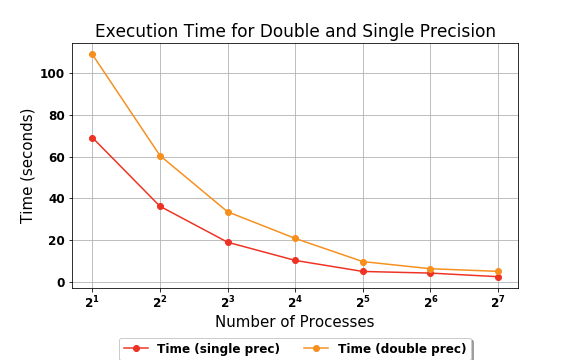
\includegraphics[width=1.\linewidth]{scaling_strong_log2.png}
		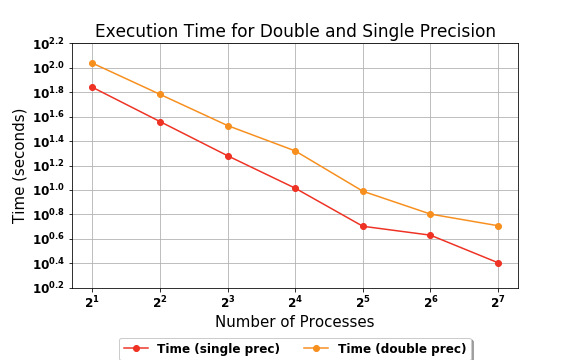
\includegraphics[width=1.\linewidth]{scaling_strong_log2log10.png}
		\caption{Strong scaling of execution time.}
		\label{fig:strong_scaling}
	\end{minipage}%
	\begin{minipage}{.5\linewidth}
		\centering
		%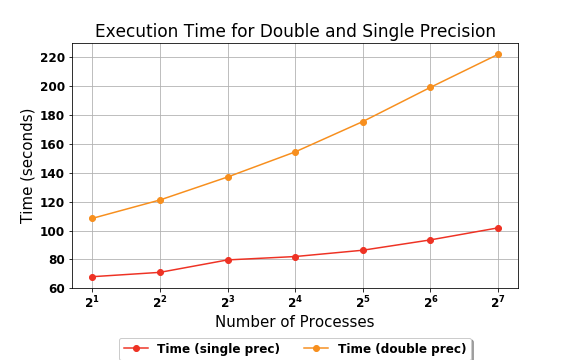
\includegraphics[width=1.\linewidth]{scaling_weak_log2.png}
		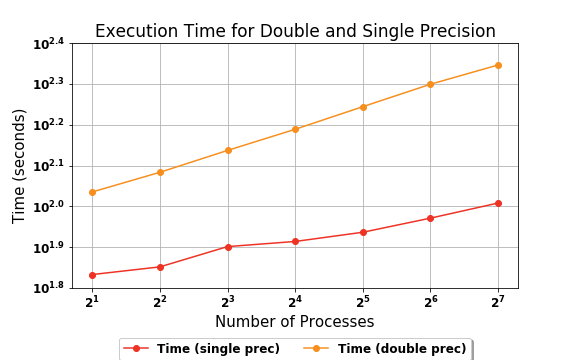
\includegraphics[width=1.\linewidth]{scaling_weak_log2log10.png}
		\caption{Weak scaling of execution time.}
		\label{fig:weak_scaling}
	\end{minipage}
\end{figure}

%---------------------------------------------------------------------------------

\subsection{Scalability Limitations}
\label{sec:scalability_limitations}
The limit on the maximum MPI message size prevented larger problem sizes being tested for the Intel Quantum Simulator. This limited the number of double precision states per process to be approximately $2^{27}$. Thus the simulator could not be tested up to the maximum available memory on a node.

To address this issue, the simulator was rebuilt using BigMPI instead of the standard MPI. However, the same problem persisted and BigMPI was later deprecated from being used with the simulator, reverting to standard MPI. As an alternative approach, Intel proposed running experiments on larger allocations on bigger European clusters, which would allow experiments using larger numbers of qubits, despite the memory on each node still being severely underutilised. To pursue this line of action, ICHEC plans on applying for a PRACE project to get the access to a larger HPC facility.

It is also noted that Intel advised that experiments with greater than two processes per node do not perform as well as for one or two processes. Thus, using many processes to fill a node's memory without exceeding the maximum MPI message size was deemed not to be a valid workaround.